\input{common.texfrag}
\usepackage{tikz}
\title{\textbf{AMLD+0 Settlement of the Geodesic Curvature-Profile Conjecture}\\[0.3em]\large Counterexample, Infinite Failure Family, and Curvature--Potential Criterion}
\author{Brian Tenneson}
\date{19 October 2026}
\begin{document}\maketitle
\begin{abstract}
We evaluate whether a minimum-edge verifier-legal directed proof path must minimize cumulative negative Ollivier--Ricci curvature burden. A six-vertex example refutes the universal claim: the unique two-edge geodesic incurs burden $1/3$, while a three-edge detour incurs zero. We reproduce exact primal and dual optimal-transport certificates, extend the failure to a leaf-amplified infinite family, and retain the bound $0\le B_-(P)\le2|P|$. A calibrated potential condition is sufficient for a geodesic to minimize curvature burden. We also provide an explicit proof-chain protocol for Horn realization, distinguish edge length from curvature burden, and state the limits of the graph-theoretic results. No proof-search performance gain follows from the geometric comparison alone.
\end{abstract}
\section{Frozen definitions and scope}
Fix a connected finite simple undirected graph $G_u=(V,E_u)$ and an orientation selecting permitted directed moves $E_{\to}\subseteq\{(x,y):\{x,y\}\in E_u\}$. Legal paths use only $E_{\to}$; Ollivier--Ricci curvature uses the underlying graph $G_u$. Let $d_u$ be its unweighted shortest-path metric and $m_x$ the uniform probability measure on the \emph{distinct neighbors} $N_u(x)$, assuming no isolated endpoint of a curvature-tested edge. For adjacent $x,y$ put
\[\kappa(x,y)=1-W_1^{d_u}(m_x,m_y),\qquad b(x,y)=\max\{0,-\kappa(x,y)\}.\]
For a finite legal directed path $P=(x_0,\dots,x_n)$ define
\[B_-(P)=\sum_{i=0}^{n-1}b(x_i,x_{i+1}),\qquad |P|=n.\]
Here a geodesic minimizes $|P|$ among legal paths with the given endpoints, \emph{not} $B_-(P)$. The conjecture under assessment asserted, without supplementary hypotheses,
\[P^*\text{ is a directed }s\text{--}t\text{ geodesic}\quad\Longrightarrow\quad B_-(P^*)\le B_-(P)\text{ for every legal }P:s\to t.\]
\section{Six-vertex counterexample and its exact certificates}
Let $V=\{s,a,t,u,v,\ell\}$. The undirected edges are
\[\{s,a\},\{a,t\},\{t,v\},\{v,u\},\{u,s\},\{a,\ell\},\]
and the legal directed edges are $s\to a\to t$, $s\to u\to v\to t$, and $a\to\ell$.

\begin{center}
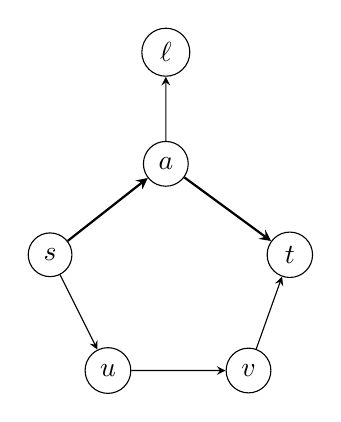
\begin{tikzpicture}[scale=1.05,every node/.style={circle,draw,minimum size=0.52cm}]
\node (s) at (-2,0) {$s$};\node (a) at (-0.6,1.1) {$a$};\node (t) at (0.9,0) {$t$};\node (v) at (0.4,-1.4) {$v$};\node (u) at (-1.3,-1.4) {$u$};\node (l) at (-0.6,2.45) {$\ell$};
\draw[->,>=stealth,thick] (s)--(a);\draw[->,>=stealth,thick] (a)--(t);\draw[->,>=stealth] (s)--(u);\draw[->,>=stealth] (u)--(v);\draw[->,>=stealth] (v)--(t);\draw[->,>=stealth] (a)--(l);
\end{tikzpicture}
\end{center}
The unique two-edge legal $s$--$t$ path is $P_g=(s,a,t)$; the detour is $P_d=(s,u,v,t)$ of length three. Thus $P_g$ is the unique geodesic.

For edge $s-a$, the neighborhood measures are
\[m_s=\tfrac12(\delta_a+\delta_u),\qquad m_a=\tfrac13(\delta_s+\delta_t+\delta_\ell).\]
A primal feasible coupling sends $1/3$ of mass $a\to\ell$, $1/6$ of $a\to t$, $1/3$ of $u\to s$, and $1/6$ of $u\to t$. The total cost is
\[\tfrac13\cdot1+\tfrac16\cdot1+\tfrac13\cdot1+\tfrac16\cdot2=\tfrac76.\]
For the dual, set $f(u)=1$, $f(s)=f(a)=f(v)=0$, and $f(t)=f(\ell)=-1$. Every graph edge changes $f$ by at most one, so $f$ is $1$-Lipschitz. Its Kantorovich--Rubinstein value is
\[\int f\,dm_s-\int f\,dm_a=\tfrac12-(-\tfrac23)=\tfrac76.\]
Primal and dual equality certify $W_1(m_s,m_a)=7/6$, hence $\kappa(s,a)=-1/6$. Reflection of the five-cycle about the leaf-bearing vertex $a$ exchanges $s$ and $t$, giving $\kappa(a,t)=-1/6$. For detour edges $s-u,u-v,v-t$, supports of the two neighbor measures have no common vertex, so all transport must cost at least one per mass unit. For $s-u$, match $a\mapsto s$ and $u\mapsto v$; for $u-v$, match $s\mapsto u$ and $v\mapsto t$; for $v-t$, match $u\mapsto v$ and $t\mapsto a$. All six matched pairs are adjacent, and every involved neighbor distribution is uniform on two vertices. These explicit couplings cost exactly one, giving $W_1=1$ and $\kappa=0$ for each detour edge. Consequently
\[\boxed{|P_g|=2<3=|P_d|,\qquad B_-(P_g)=\tfrac13>0=B_-(P_d).}\]
This refutes the stated universal graph-theoretic conjecture.

\begin{remark}[Explicit verifier-legal realization]
To avoid assuming that every abstract directed graph automatically arises as a genuine theorem graph, choose propositional atoms $p_x$ for each $x\in V$, frozen assumptions $\Gamma=\{p_s\}\cup\{p_x\to p_y:(x,y)\in E_{\to}\}$, and a fixed protocol allowing one edge transition precisely by applying the indicated Horn implication to its antecedent. Every directed path corresponds to a legal sequence of independently checkable modus-ponens steps from $p_s$ toward $p_t$. Here a protocol state tracks one current active atom $p_x$ and the unchanged finite axiom table, rather than the full monotonically accumulated consequence BANK. A permitted step checks one recorded implication $p_x\to p_y$ and its single modus-ponens application, updates the active atom to $p_y$, and charges one edge; all checked implications remain frozen. This implements the directed \emph{path protocol} used in the theorem. A general proof calculus might combine previous discoveries or use macros to add new transitions, so the conclusion is not asserted for its unrestricted proof-state graph.
\end{remark}

\section{Infinite leaf-amplified failure family}
For each integer $r\ge2$, replace $\ell$ with leaves $\ell_1,\dots,\ell_r$ adjacent only to $a$, and direct the new leaf edges outward from $a$. Set $q=r+2$. At $s-a$, source masses remain $m_s=\frac12(\delta_a+\delta_u)$ and target demands are $1/q$ at each of $s,t,\ell_1,\ldots,\ell_r$. For $r\ge2$, send $1/2$ mass from $a$ to the leaves (distance one); send $1/q$ from $u$ to $s$ (distance one), $1/q$ to $t$ (distance two), and the remainder $1/2-2/q$ to leaves (distance three). Its cost is
\[\tfrac12+\tfrac1q+\tfrac2q+3\bigl(\tfrac12-\tfrac2q\bigr)=2-\tfrac3q.\]
A matching dual potential is
\[f(u)=1,\quad f(s)=f(v)=0,\quad f(a)=f(t)=-1,\quad f(\ell_j)=-2\quad(1\le j\le r).\]
It is $1$-Lipschitz on the full undirected graph and its dual objective is $2-3/q$. Thus
\[\kappa(s,a)=\kappa(a,t)=-\frac{r-1}{r+2},\quad B_-(P_g)=\frac{2(r-1)}{r+2},\quad B_-(P_d)=0,\quad \lim_{r\to\infty}B_-(P_g)=2.\]
The $r=1$ six-vertex example was computed separately above; the displayed $r\ge2$ coupling must not be extrapolated to $r=1$. Adding the leaves changes local neighborhood geometry while leaving both directed route lengths fixed, establishing the off-path neighborhood obstruction.

\section{Universal curvature-burden bound}
\begin{theorem}\label{thm:bound}
For every adjacent pair $x,y$ in an unweighted undirected graph with neighbor measures as above, $-2\le\kappa(x,y)\le1$. Every $n$-edge verifier-legal path therefore satisfies $0\le B_-(P)\le2n$, and every directed geodesic $P_g$ from $s$ to $t$ satisfies $B_-(P_g)\le2d_{\to}(s,t)$.
\end{theorem}
\begin{proof}
For $z\in N_u(x)$ and $w\in N_u(y)$, the walk $z-x-y-w$ has length at most three. Hence all couplings between $m_x$ and $m_y$ cost at most three and $0\le W_1\le3$. Rearrangement gives the curvature bound; summing nonnegative edge burdens gives $B_-\le2n$. For a directed geodesic $n=d_{\to}(s,t)$.
\end{proof}

\section{A curvature--potential bridge, with its exact scope}
\begin{theorem}[Curvature--Potential Geodesic Bridge]\label{thm:bridge}
Fix reachable vertices $s,t$. Suppose there exist $\alpha\ge0$ and a function $\phi:V\to\R$ such that every legal directed edge satisfies
\[b(x,y)\ge\alpha+\phi(x)-\phi(y).\]
If a directed \emph{length geodesic} $P_g$ from $s$ to $t$ attains equality on \emph{each edge}, then $P_g$ minimizes total negative-curvature burden among all legal $s$--$t$ paths.
\end{theorem}
\begin{proof}
For any legal $P:s\to t$ telescope the edge inequalities to get $B_-(P)\ge\alpha|P|+\phi(s)-\phi(t)$. Since $|P|\ge |P_g|$ and $\alpha\ge0$, this is at least $\alpha|P_g|+\phi(s)-\phi(t)$. Equality on all edges of $P_g$ makes the latter expression $B_-(P_g)$.
\end{proof}
\begin{remark}
The condition permits $\alpha=0$. The existence of a calibrated potential saturating a chosen geodesic is a \emph{substantive additional hypothesis}, not inferred from geodesicity or curvature. The bridge is an optimality certificate of a familiar potential/telescoping kind, not an algorithm for constructing $\phi$, and does not imply the proposed AMLD search policy will discover the route.
\end{remark}

\section{Interpretation, reproducible checks, and boundaries}
Local curvature is not determined by vertex degree alone: an edge of a triangle $K_3$ has $\kappa=1/2$, while a cycle edge of $C_5$ has $\kappa=0$, although both examples have degree-two endpoints and unit edge length. Graph curvature describes local transportation geometry; legal proof distance is global and directed.

The displayed exact transport couplings and dual functions constitute mathematical optimality certificates. Additional exact rational min-cost-flow computations agreed with the formulas for $r=1,\dots,12$, but finite checks do not replace the symbolic proof. No claim is made that six vertices is the minimum possible number for a counterexample; that would require a separate exhaustive argument. A topological graph may serve as a proof-step protocol only after its allowed edges and verification receipts have been fixed. The construction does not apply automatically to unrestricted proof calculi.

\paragraph{Settlement classification.} The universal strong conjecture is \textsf{REFUTED} in the graph and the specified Horn step protocol. Theorems~\ref{thm:bound} and~\ref{thm:bridge} remain conditional positive results. Whether curvature profiles statistically predict short or useful proofs in a real prover is untested here. The stated mathematical counterexample does not imply that six independent AMLD or FORGE-6 agents have executed the corresponding search.

\paragraph{Scope.} The infinite-family coupling is stated for $r\ge2$, the potential bridge requires edgewise saturation along the chosen geodesic, and the Horn realization concerns the declared path protocol, not every possible proof-search policy.
\end{document}
